\titlespacing{\chapter} {0pt}{0pt}{0pt}
\chapter{Lung Cancer} 
\ifpdf
    \graphicspath{{Chapter1/figures/}}
\else
    \graphicspath{{Chapter1/figures/}}
\fi

\titlespacing{\section} {0pt}{0pt}{0pt}
\section{See Steven's email 22/10/15}

\section{Epidemiology}
Lung cancer is a disease with an ever increasing global burden, contributing to more than 1.5 million deaths world wide in 2010\supercite{Lozano:2012kd} and 2.5 million new diagnoses\supercite{Jemal:2008df} with an incidence of nearly 500 per 100000\supercite{Boyle:2008va}. Traditionally, lung cancer has a far higher incidence amongst men than women, however in Australia, from 1982 - 2011 that difference has diminished from over 4 fold to under 2 fold (Fig. \ref{figIncidence})\supercite{AIHW:2015tp}. This change is due, not only to the falling incidence of lung cancer amongst men, but also to the rising incidence amongst women. 
% obtained from excel file from AIHW source 
\begin{figure}[h] %h == float figure
	\centering
	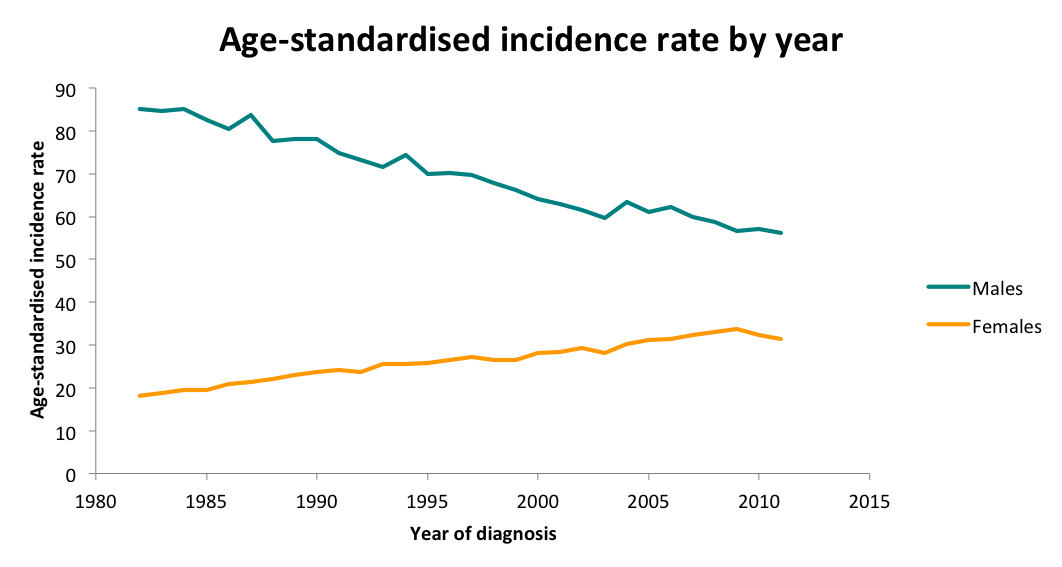
\includegraphics[width=0.75\textwidth]{incidence.png}
	\caption{Lung Cancer Incidence in Australia, 1982 - 2011}
	\label{figIncidence}
\end{figure}


\section{Aetiology}
In 1964, it was first recognised that cigarette smoke was casually related to lung cancer, with a report to the Surgeon General of America concluding "the magnitude of the effect of cigarette smoking [on lung cancer] far outweighs all other factors"\supercite{Service:1976tz}. The changing incidence in lung cancer reflects the current Australian societal trend in falling smoking prevalence, amongst both men and women. In 1980 41~\% of men and 30~\% of women were classified as regular smokers (smoking at least weekly), nearly converging at 22~\% and 18~\%, respectively, in 2010\supercite{Scollo:2013vj}. 

\section{Histopathology}
Previously lung cancer was simply divided in to non-small cell lung cancer (NSCLCa)\nomenclature{$NSCLCa$}{non-small cell lung cancer} and small cell lung cancer (SCLCa)\nomenclature{$SCLCa$}{small cell lung cancer}, but as the understanding of lung cancer has developed is now possible, and required, to further differentiate lung cancer in to the various distinct but related subtypes.

Approximately 85~\% of lung cancers are NSCLCa\supercite{Herbst:2008fv} which can then be subsequently further divided in to the following three major distinct histological subtypes\supercite{Travis:2004ti}; adenocarcinoma, squamous cell carcinoma (SqCCa)\nomenclature{$SqCCa$}{squamous cell carcinoma} and large cell carcinoma (LCC)\nomenclature{$LCC$}{large cell carcinoma}. From 1980 to 1997 a shift in NSCLCa histopathologies was identified with an increase in the incidence of adenocarcinomas and a fall in the incidence of squamous cell carcinoma\supercite{Devesa:2005jw}. 

\section{Mutation}
All malignancies are thought to arise from a single or series of genetic mutations which then confer an ability to replicate in an uncontrolled manner. 
In 2004 it was identified that 10~\% of patients with NSCLCa will have a, potentially dramatic, response to tyrosine kinase inhibitors (TKI)\nomenclature{$TKI$}{Tyrosine Kinase Inhibitors}\supercite{Lynch:2004ii}. Since then the Catalogue of Somatic Mutations in Cancer (COSMIC)\footnote{http://cancer.sanger.ac.uk/cosmic}\nomenclature{$COSMIC$}{Catalogue of Somatic Mutations in Cancer} database\supercite{Forbes:2015gp} lists over 26000 different mutations, with 4600 having a frequency of greater than 1~\%. 

Since then 145 genes have been identified as potential lung cancer driver mutations\supercite{Chen:2013kz}, however only a few currently possess commercially available therapeutic drugs. 

\subsection{EGFR}

The Epidermal Growth Factor Receptor (EGFR)\nomenclature{$EGFR$}{Epidermal Growth Factor Receptor} is a 170 kdalton member of the ErbB family of cell surface tyrosine kinases\supercite{Cadranel:2013fl}, and is encoded on chromosome 7. The receptor belongs to the HER/erbB  family of tyrosine kinases, which include HER1 (EGFR/erbB1), HER2 (neu, erbB2), HER3 (erbB3) and HER4 (erbB4)\supercite{daCunhaSantos:2011jb}. 

The EGFR is made of up three portions; an extracellular ligand binding domain, a transmembrane domain and an intracellular tyrosine kinase domain\supercite{Krause:2005fa, Yarden:2001ta}. Activation of the protein is achieved by binding of a ligand (such as epidermal growth factor, transforming growth \mbox{factor-\textalpha} and neureguelins\supercite{Yarden:2001ta}) to the extracellular domain. Once a ligand is bound to the extracellular domain, the receptor undergoes dimerisation or heterodimerisation with related receptors (especially HER2/neu\supercite{Tzahar:1996us}). Without the aforementioned ligand binding and subsequent dimerisation, there is no intrinsic activity of the tyrosine kinase portion of the receptor\supercite{Yarden:2001ta}. 

The tyrosine kinase portion of the receptor is normally in a state of autoinhibition, but on dimerisation there is rapid autoposphorylation of the intracellular tyrosine residues. The phosphorylated then functions to allow assembly and activation of intracellular messenger proteins\supercite{Lemmon:2010bq, Cohen:1981th}, especially through the mammalian target of rapamycin (mTOR)\nomenclature{$mTOR$}{Mammalian target of rapamycin}\supercite{Siegelin:2014jj}. 

In 1984 Gill \textit{et al} demonstrated that EGFR blockade with a chimeric anti-EGFR antibody, in human epidermoid carcinoma cell lines expressing EGFR, resulted in a reduction in \mbox{auto-posphorylation}\supercite{Gill:1984wv}. A similar study by Kawamoto \textit{et al} revealed a biphasic cell proliferation response to the same cells exposed to Epidermal Growth Factor (EGF)\nomenclature{$EGF$}{Epidermal Growth Factor}; with cellular proliferation at low levels of EGF and inhibition at higher levels. Taken together, this was felt to demonstrate that in human epidermoid malignancies EGFR expression and activation played a role in  cancer proliferation. 

Over expression of \textit{EGFR} \textbf{(?need to add gene here)} has been identified in a variety of cancers including: head and neck, ovarian, bladder, oesophageal, gastric, brain, breast, endometrial, colonic and lung\supercite{Sharma:2007dx}. In NSCLCa, \textit{EGFR} overexpression has been identified in 41~\% of adenocarcinomas\supercite{Lynch:2004ii} and 89~\% of squamous cell carcinomas (SqCCa)\supercite{AlOlayan:2012dx}\nomenclature{$SqCCa$}{Squamous cell carcinoma}. 

As \textit{EGFR} was noted to be overexpressed in NSCLCa\supercite{Lynch:2004ii, AlOlayan:2012dx} and blockade with monoclonal antibodies\supercite{Gill:1984wv} resulted in cell line response, it was felt that a targetted EGFR tyrosine kinase inhibitor, gefitonib, might have produced anti-tumoural activity. While initial studies demonstrated (Multi-Institutional Randomized Phase II Trial of Gefitinib for
Previously Treated Patients With Advanced Non–Small-Cell
Lung Cancer) response, docetaxel vs gefitonib where less promising, in advanced NSCLCa already pre-treated.  

\subsubsection{T790M}

\subsection{KRAS}

\subsection{ALK / ROS1 Rearrnagment}

\section{Prognosis}

\subsection{Early Stage}
Surgery for early NSCLCa provides a potentially currative management strategy. However, even for those patients who receive currative intent surgical resection, followed by optimal adjuvant chemotherapy (when appropriate) will only receive an absolute overall survival (OS)\nomenclature{$OS$}{overall survival} advantage of 5.4~\% at 5 years and an improvement in disease free survival\nomenclature{$DFS$}{disease free survival} of 5.8~\%\supercite{Pignon:2008ep}. This equates to a 5 year survival rate for NSCLCa, depending pathological stage, from 25~\% to 73~\%\supercite{FRCS:2011ip}.

\subsection{Late Stage}
However, over 75~\% of patients with new NSCLCa diagnoses will present with an advanced stage\supercite{Slatore:2011hf}, and will not be eligible for currative intent treatment. Those presenting thusly will have a median survival of only 119 days\supercite{Rapp:1988uh} without chemotherapy. Even those patients who are suitable to receive conventional chemotherapy, an overall survival of only about 8 months is achievable with a response rate of only 19~\% achievable\supercite{Schiller:2002gi}.

\section{Diagnosis}

Foobar\supercite{Schiller:2002gi}.

\subsection{Radiology}
\subsection{Tissue Obtaining}
Difficultly obtaining tissue
Earlier diagnosis == smaller nodules 
Smaller tissue == less to analyse == less DNA to use

\section{Tissue analysis}
\subsection{current methods}
\subsection{next gen sequencing}